\documentclass{article}
\usepackage[utf8]{inputenc}
\usepackage[spanish]{babel}
\usepackage{listings}
\usepackage{graphicx}
\graphicspath{ {images/} }
\usepackage{cite}

\begin{document}

\begin{titlepage}
    \begin{center}
        \vspace*{1cm}
            
        \Huge
        \textbf{Proyecto de Investigación}
            
        \vspace{0.5cm}
        \LARGE
        Taller Noción de la memoria del computador
            
        \vspace{1.5cm}
            
        \textbf{Maria Cristina Vergara Quinchia}
            
        \vfill
            
        \vspace{0.8cm}
            
        \Large
        Despartamento de Ingeniería Electrónica y Telecomunicaciones\\
        Universidad de Antioquia\\
        Medellín\\
        Septiembre de 2020
            
    \end{center}
\end{titlepage}

\tableofcontents
\newpage
\section{Introducción}\label{intro}
Si bien la mayoría de personas ya estamos familiarizadas con las palabra  “memoria", que se  define cómo la capacidad para recordar o retener información,se puede formular la siguiente pregunta:que relación tendría la palabra memoria con un computador?Algunos tienen una leve noción de que es y para que sirve este componente dentro de un dispositivo electrónico,en este trabajo se va a abordar el papel que juega la memoria dentro de un computador y se hablará sobre su concepto,su funcionamiento,los tipos de memorias y sus diferencias.
\section{Contenido}\label{contenido}
A continuación se desarrollarán los puntos propuestos en el taller.

\subsection{Defina que es la memoria del computador.}
 “Las memorias son los dispositivos de almacenamiento de datos e instrucciones en una computadora”\cite{UNT}.
La memoria del computador es un dispositivo que guarda la información de forma temporal o sea que almacena información durante un periodo de tiempo,esta información puede ser accedida  por el procesador para ejecutar las instrucciones y realizar las tareas de forma rápida y eficiente.
También se podría definir como “un conjunto de celdas de almacenamiento junto con los circuitos asociados que se necesitan para ingresar y sacar la información de almacenamiento”\cite{FIng}.

\subsection{Mencione los tipos de memoria que conoce y haga una pequeña descripción de cada tipo.}
Los computadores utilizan varios tipos de memoria con diferentes funciones y características como la velocidad y la capacidad de almacenamiento, las más conocidas son:
\begin{itemize}
\item \textbf{Memoria Caché}:
    En la memoria caché se almacena una copia de la memoria RAM,dicha copia contiene la información que  emplea el procesador frecuentemente para ejecutar las ordenes, lo cuál reduce el tiempo en el que se obtiene y se transfiere la información ya que el procesador no tiene que ir a buscarla se puede decir que la obtiene de forma casi inmediata.Esto de debe a que la memoria caché se encuentra localizada dentro del procesador y consta de tres niveles Nivel 1,Nivel 2 y Nivel 3.A medida que se asciende en el nivel de la memoria caché la capacidad aumenta y la velocidad disminuye en cada nivel.La capacidad de esta memoria  es de 12 Megabytes aproximadamente y aunque tiene menos capacidad que la memoria RAM es mucho más costosa y rápida\cite{ref}.\newline
    Están diseñadas para reducir el tiempo de acceso a la memoria. En la memoria caché se almacenan los datos que se prevé que se utilizarán más habitualmente, de manera que sea posible reducir el número de accesos que debe hacer el procesador a la memoria principal (ya que el tiempo de acceso a la memoria principal siempre es superior al tiempo de acceso a la memoria caché)\cite{Orenga}.

    \item \textbf{Memoria RAM(Ramdom Access Memory): }En español Memoria de Acceso Aleatorio,se podría decir que esta es la más conocida por ser la memoria principal del computador.Se caracteriza por ser de lectura/escritura,puede leer y modificar la información,es volátil o sea que su información se pierde cuando no hay suministro de energía.\newline
    La memoria RAM, también llamada memoria principal, por ser la principal conexión con el microprocesador, es físicamente un circuito electrónico compuesto por un grupo de chips que se conectan a la Motherboard por una serie de contactos en su base. Cada uno de los chips que componen la memoria es una unidad que se divide en celdas, siendo posibles de ser accedidas a través de una dirección que las identifica\cite{ram}.\newline
    En cada celda de la memoria se almacena la información temporalmente,la falta de información se puede representar con un 0,por el contrario la existencia de información en dicha celda se puede representar como un 1.Actualmente se pueden encontrar memorias RAM de hasta 32 Gigabytes de almacenamiento.\newline
    Se puede clasificar en:
    \begin{itemize}
    \item\textbf{DRAM(Dynamic Random Access Memory):}En español memoria dinámica de acceso aleatorio.En cada celda de esta memoria se están compuestas por un capacitor y un transistor,los capacitores contienen la información y los transistores recargan las celdas continuamente para mantener los datos y evitar que se pierdan.El proceso de recargar las celdas repetitivamente hace que sea una memoria lenta aún así tiene buen espacio de almacenamiento y son asequibles.
    \item\textbf{SRAM(Static Random Access Memory):}En español memoria estática de acceso aleatorio.Cada celda de esta memoria consta de 4 o 6 transistores y algunos circuitos,esto hace que en la memoria no se requiera estar recargando las celdas continuamente.Esta memoria es más rápida que la anterior pero  tiene menos capacidad de almacenamiento y costos más elevados\cite{ref1}. 
        
    \end{itemize}
    
    En la Figura (\ref{fig:memoria}), se puede observar una memoria RAM.
     \begin{figure}[h]
    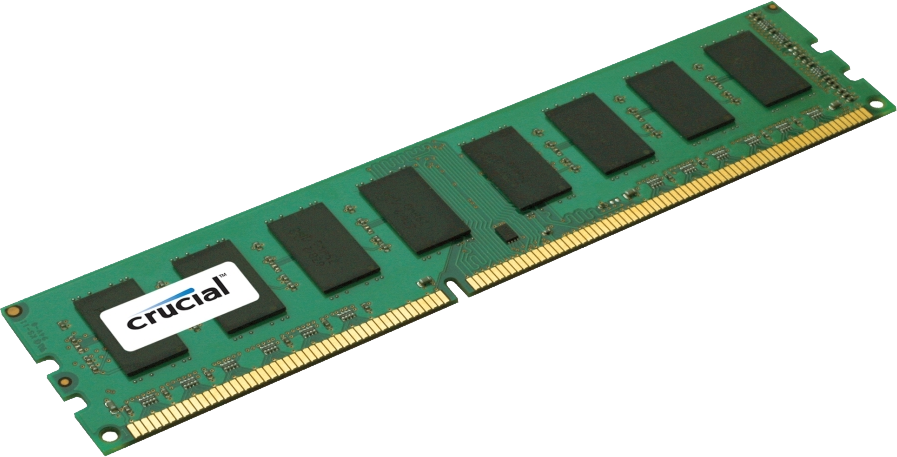
\includegraphics[width=4cm]{memoria.png}
    \centering
    \caption{Memoria RAM}
    \label{fig:memoria}
    \end{figure}
    
    
    
    \item \textbf{Memoria ROM(Read Only Memory)}: En español Memoria de sólo lectura,esta memoria lee la información sin poder modificarla o eliminarla,es una memoria no volátil lo que quiere decir que su información permanece aún si no hay fuente de energía.\newline
    Estas memorias una vez programadas sólo realizan operaciones de lectura. No son volátiles pueden utilizarse para almacenar códigos, generadoras de caracteres, funciones aritméticas complejas, unidades de control microprogramadas, almacenamiento de partes del sistema operativo (BIOS), entre otras\cite{refUNT}.
    
    En la Figura (\ref{fig:rom}), se puede observar una memoria ROM.
    \begin{figure}[h]
    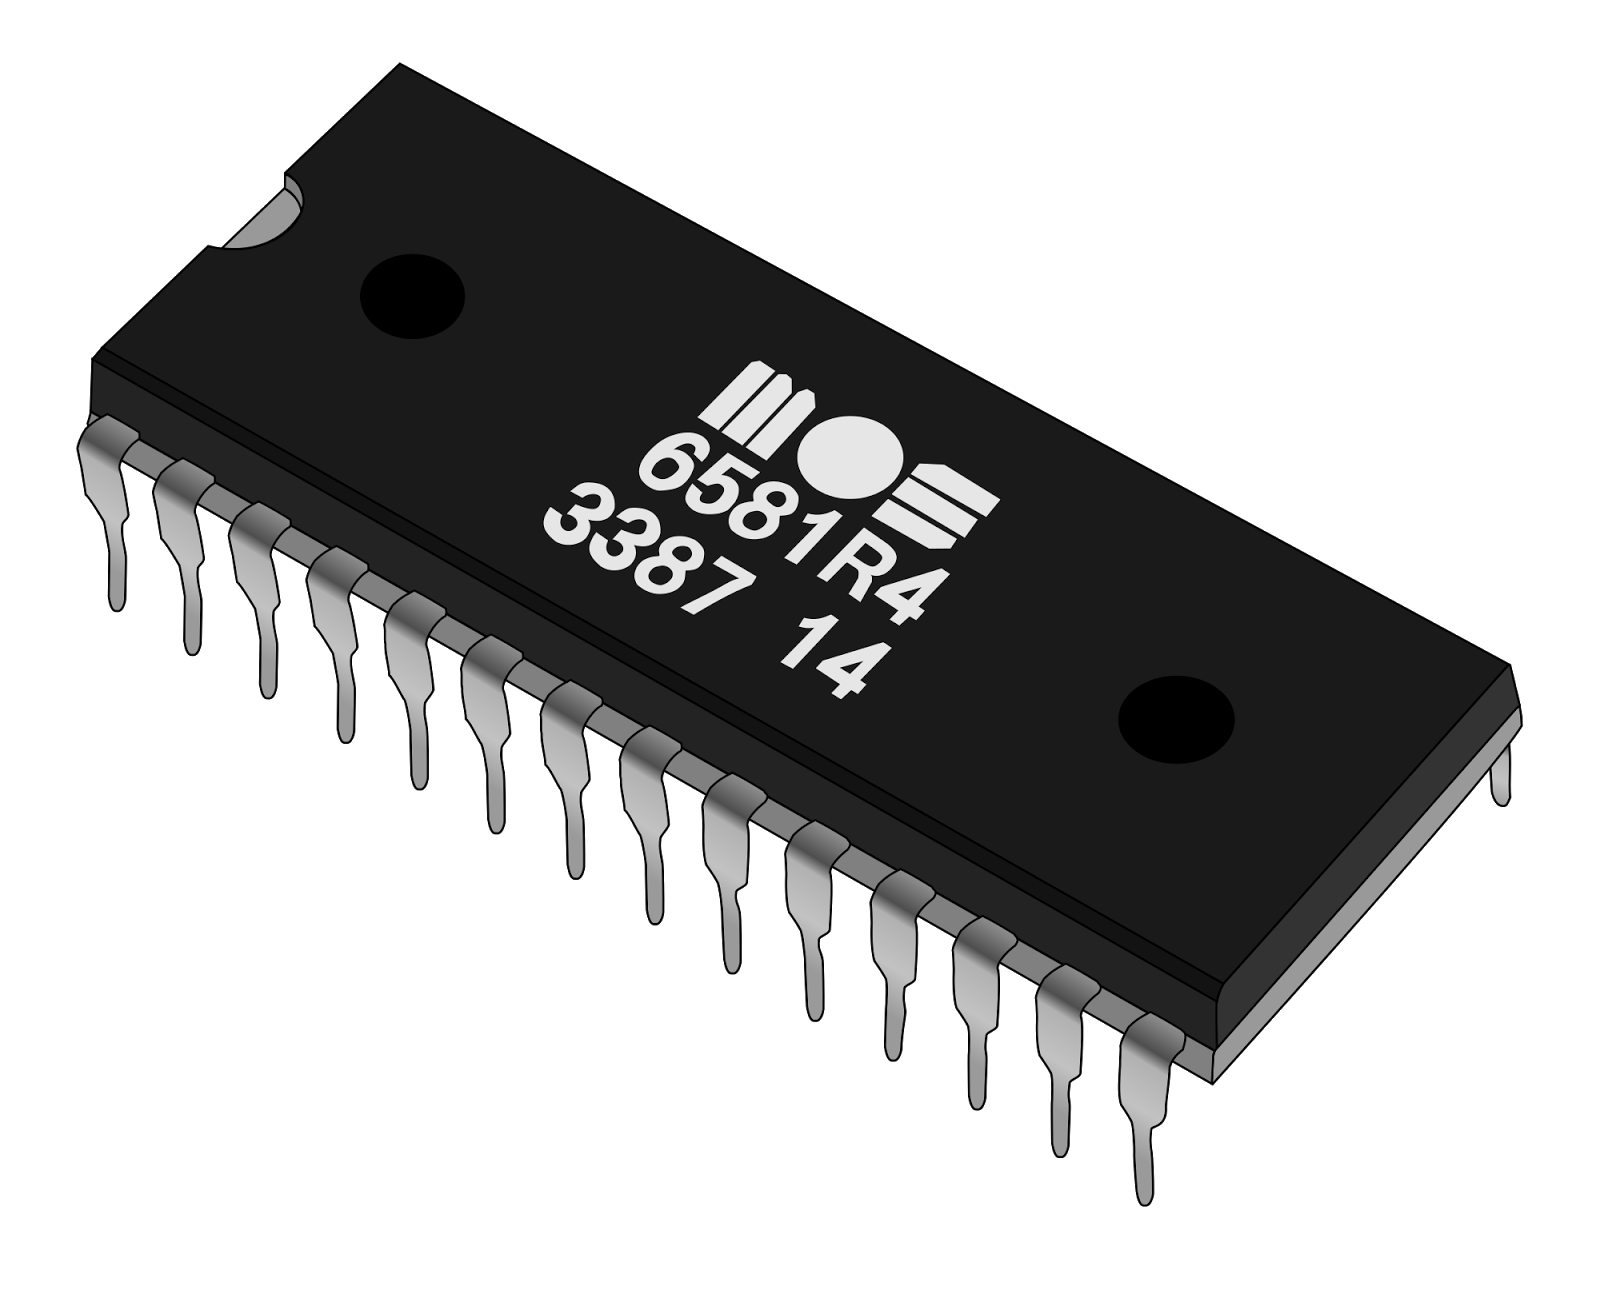
\includegraphics[width=4cm]{rom.png}
    \centering
    \caption{Memoria ROM}
    \label{fig:rom}
    \end{figure}
    
    
\end{itemize}


\subsection{Describa la manera como se gestiona la memoria en un computador.}
Se podría decir que la gestión  de la memoria se hace tanto en el hardware cómo en el software.A través del controlador de memoria (Centro de Control de Memoria),ubicado en la placa madre o en el procesador del computador.
Este controlador interviene en la transferencia de información entre los dispositivos,gestiona la velocidad y capacidad de la memoria,hace una revisión en cada una de la sus celdas para encontrar posibles fallos.
En las memorias DRAM el controlador recarga los capacitores en las celdas para evitar que se descarguen y se pierda la información\cite{ref2}.
Respecto a software el sistema operativo también  hace su gestión de la memoria en conjunto con el controlador repartiendo el almacenamiento disponible para procesos que se estén ejecutando al mismo tiempo asignando a cada uno una porción de memoria.\cite{gm}.\newline
 En los sistemas operativos modernos la
gestión de memoria resuelve aspectos como:
\begin{itemize}
    \item {La carga de programas y su ubicación. Hay que establecer la correspondencia
entre las direcciones lógicas del programa y su ubicación física en memoria.}
\item{ La presencia simultánea de más de un programa en memoria.}

\item{ La compartición de espacios de memoria por varios programas.}

\item{ La ejecución de programas que no caben completos en memoria.}
\item{ La gestión eficiente del espacio de memoria libre}\cite{gestion}.
\end{itemize}







\subsection{¿Qué hace que una memoria sea más rápida que otra? ¿Por qué esto es importante?}

Lo que hace una que una memoria sea más rápida que otra es la disminución de la latencia(retardo o intervalo de tiempo en el que se  accede a la información de la memoria),entre menos sea la latencia mayor es la velocidad,por ejemplo en las memorias que están dentro del procesador(caché) la latencia es mínima,por el contrario las memorias externas al  procesador como la memoria RAM,  la latencia suele a aumentar debido a que  la información se tiene que transmitir de un componente a otro. 
Es importante  porque entre más reducida sea la latencia,la memoria será más rápida y eficiente en la lectura,escritura y transferencia de datos lo que aportaría al buen rendimiento del sistema.\newpage




\section{Conclusiones}
\begin{itemize}
    \item{Las memorias  rápidas como la memoria caché,tienen altos costos y menor capacidad de almacenamiento mientras que las memorias lentas son asequibles y tienen mayor capacidad de almacenamiento. }
    \item{El procesador no prefiere trabajar con el disco duro,prefiere trabajar con la memoria RAM ya que con esta  accede a la información con mayor rapidez.}
    \item{En la memoria se operan grandes cantidades de información debido a que el procesador no posee suficiente espacio de almacenamiento para hacerlo. }
\end{itemize}




\newpage
    


\bibliographystyle{IEEEtran}
\bibliography{references}


\end{document}

